% This is a LaTeX thesis template for Monash University.
% to be used with Rmarkdown
% This template was produced by Rob Hyndman
% Version: 6 September 2016

\documentclass{monashthesis}

%%%%%%%%%%%%%%%%%%%%%%%%%%%%%%%%%%%%%%%%%%%%%%%%%%%%%%%%%%%%%%%
% Add any LaTeX packages and other preamble here if required
%%%%%%%%%%%%%%%%%%%%%%%%%%%%%%%%%%%%%%%%%%%%%%%%%%%%%%%%%%%%%%%

\author{Huize Zhang}
\title{Thesis title}
\studentid{27478343}
\def\degreetitle{Bachelor of Commerce (Honours)}
% Add subject and keywords below
\hypersetup{
     %pdfsubject={The Subject},
     %pdfkeywords={Some Keywords},
     pdfauthor={Huize Zhang},
     pdftitle={Thesis title},
     pdfproducer={Bookdown with LaTeX}
}


\bibliography{thesisrefs}

\begin{document}

\pagenumbering{roman}

\titlepage

{\setstretch{1.2}\sf\tighttoc\doublespacing}

\clearpage\pagenumbering{arabic}\setcounter{page}{0}

\hypertarget{ch:intro}{%
\chapter{Introduction}\label{ch:intro}}

Decisions by courtroom Justices have been discussed broadly in the legal literature. Gender, political views and religious background of both the Justices and counsel in the case potentially influence the decisions. This paper will explore the facial behaviour of the Justices during hearings with the objective of being to assess whether it can help to predict outcomes. Audio Visual(AV) recordings and case transcripts will be computationally processed and analysed to examine the decisions of each Justice.

\hypertarget{motivation}{%
\section{Motivation}\label{motivation}}

\textcite{tutton2018judicial} attemped to utilize the AV technology, which is made available online by the High Court of Australia \autocite{highcourtau}. They visually inspect of the videos to highlight when Justices depart from the expected norms of judicial conduct. To better understand the emotion status and therefore the departure of the emotional behaviour, more advanced technologies could be applied. An example is to use OpenFace \autocite*{baltrusaitis2018openface} technology, which provides information on emotions exhibited by the Justices. This technique has been applied by \textcite{kovalchik2018going} on professional tennis players during Grand Slam matches. That study demonstrated the potential to predict the outcome of High Court appeals based on Justices' demeanour utilising contemporary tools and emotion tagging techniques.

\hypertarget{literature-review}{%
\section{Literature review}\label{literature-review}}

The literature sumary is divided into two parts: (1) current work in legal studies to understand the behaviour of the Justices and (2) existing facial recognition and emotion tagging technology.

\hypertarget{legal-study-from-a-behaviour-perspective}{%
\subsection{Legal study from a behaviour perspective}\label{legal-study-from-a-behaviour-perspective}}

People have attempted to predict the decisions of the Justices for centuries. \textcite{judicalguid} present the following code of conduct:

\begin{quote}
It is important for judges to maintain a standard of behaviour in court that is consistent with the status of judicial office and does not diminish the confidence of litigants in particular, and the public in general, in the ability, the integrity, the impartiality and the independence of the judge.
\end{quote}

This impartiality should be clear in judicial demeanour \autocites{tutton2018judicial}{goffman1956nature}. Paul Ekman \autocite{ekman1991invited} suggests that from a behavioural perspective, some facial and vocal inflections are often unbeknown to the speakers themselves . Many scholars have exploited this in studying the court outcomes through the language and words used by the Justices in the court \autocite{Shullman2004illusion} and vocal and facial characteristics of the Justices \autocite{chen2018justice}.

There are also existing works to understand the emotion of the Justices from a linguistic perspective and suggest some factors that could be useful to indicate how the Justices' vote and thus the court outcome. These factors include the use of pleasant and unpleasant language by \textcite{black2011emotions}, the frequency and content of Justices' questions by \textcite{Shullman2004illusion} and \textcite{johnson2009inquiring}. \textcite{epstein2010inferring} use a regression analysis with the number of questions asked by the Justices used to infer the winning party in a case.

Other scholars \autocites{chen2016perceived}{chen2017covering}{schubert1992observing} have studied the emotion of the Justices from vocal characteristics and suggest that these vocal characteristics, especially perceived masculinity is strongly correlated with the court outcomes. \textcite{dietrich2019emotional} uses a multilevel logistic model with random effects to suggest that subconscious vocal inflections contain information that is not available from text.

Chen \autocite*{chen2018justice} employed both vocal and facial characteristics to predict the court votes using Supreme Court data from 1946-2014. The audio clips are first preprocessed to get the Mel-frequency Cepstral Coefficients (MFCC) and then applied to a random forest model. The image features are extracted using a Histogram of Oriented Gradients (HOG) method. More specific facial recognition software is readily available to extract human facial features and these facial recognition technologies have not yet been applied to the legal proceedings.

Most of the literature is conducted using the U.S. Supreme Court Database and less studies have been conducted using Australian High Court data. \textcite{tutton2018judicial} have used an ethnographic approach to study the transcript and AV recordings in the High Court of Australia but the study is conducted in an observational manner via matching the Justices' distinct behaviour with the transcript.

\hypertarget{facial-recognition}{%
\subsection{Facial recognition}\label{facial-recognition}}

An anatomical analysis of facial action \autocite{ekman1976measuring} led to the Facial Action Code (FAC) \autocite{ekman1978} and has been further revised by \textcite{ekman2002facial}. This decomposition of facial muscles is widely used in scientific research. It was applied in competitive sports, specifically tennis by \textcite{kovalchik2018going} who found that the emotion of professional tennis players will have an impact on their performance.

There have been many algorithms created for facial detection and the analysis of their performance when applied to images have been the focus of events like the Audio/Visual Emotion Challenge \autocites{schuller2012avec}{schuller2011avec} and Emotion Recognition In The Wild Challenge and Workshop \autocites{dhall2013emotion}{kahou2013combining}.

Facial recognition software has also been implemented by DeepFace \autocite{taigman2014deepface} from Facebook, and FaceNet \autocite{schroff2015facenet} from Google. OpenFace \autocite{baltrusaitis2018openface} is the first open-sourced face recognition software that provides facial expression detection, including facial landmarking, head pose estimation, eye gaze tracking and facial action unit detection. Along with its previous version (\textcite{baltruvsaitis2016openface}), the OpenFace toolkit has been used in different social research studies including depression classification (\textcite{yang2016decision} and \textcite{nasir2016multimodal}).

\hypertarget{data-source}{%
\chapter{Data Source}\label{data-source}}

\hypertarget{data-processing}{%
\section{Data Processing}\label{data-processing}}

The source data for this research project is the AV recordings publicly available from the High Court of Australia \autocite{highcourtau}. Multiple procedures need to be performed to obtain the dataset.

The workflow for extracting numerical data from the videos can be found in Figure \ref{fig:workflow}. Youtube-dl \autocite{youtube-dl} has been used to download videos from the High Court of Australia\autocite{highcourtau} and the list of videos used in this research project is documented in the Appendix. Image frames are extracted from the videos for every minute via ffmpeg \autocite{ffmpeg}, resulting in 1021 image frames (252 frames from \texttt{Nauru} videos and 769 frames from other five videos). Taipan \autocite{Taipan} is then used to find the x-y coordinates of the location of the Justices in each image frame. ImageMagick \autocite{ImageMagick} is then used to crop the face of each Justice from each image frame that is taken from each video where three Justices present in \texttt{Nauru} videos and five Justices in other videos. The resulting 4601 cropped images (252 image frames from \texttt{Nauru} videos where three Justices are presented and 769 image frames from other videos where five justices are presented) are then sent to OpenFace \autocite{baltrusaitis2018openface} to produce the variables for facial landmarking, head pose, eye gaze and facial action unit. This step is performed via the docker platform. The resulting outputs from OpenFace are individual comma-separated values (csv) files for each of the 4601 faces considered and processing is done in R to combine all the separate csv files into a final dataframe with appropriate index of \texttt{frame\_id}, \texttt{judge\_id} and \texttt{video\_id}.

\begin{figure}
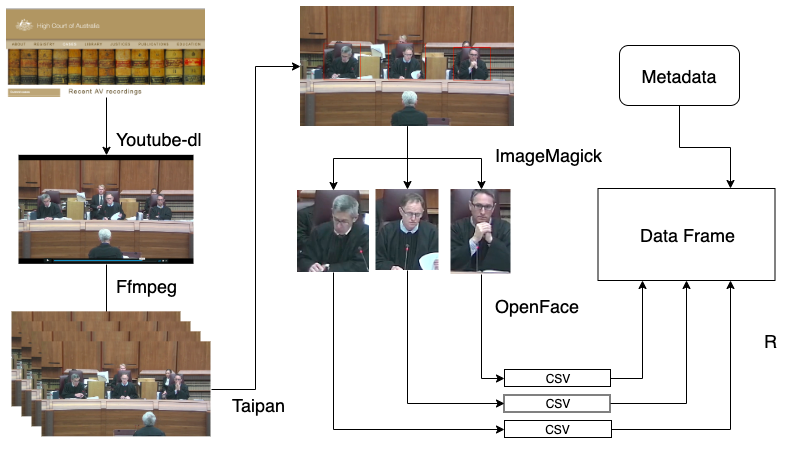
\includegraphics[width=6.2in]{figures/workflow} \caption{workflow \label{fig:workflow}}\label{fig:unnamed-chunk-1}
\end{figure}

\hypertarget{variable-description}{%
\section{Variable description}\label{variable-description}}

OpenFace provides more than 711 variables measuring different aspect of a given face and a full description of the output variables can be found \href{https://github.com/TadasBaltrusaitis/OpenFace/wiki/Action-Units}{here}. This outlines the difficulty of this project: no existing models will present accurate prediction and inference using 700+ variables - how can we incorporate these information to say about the facial expressions of the Justices during the hearings?

I conduct some exploratory data analysis on one video: \texttt{Nauru\_a} and find the 700+ variables can be classified as follows with some insights

\begin{itemize}
\item
  \textbf{Confidence}: How confidence OpenFace is with the detection. Confidence is related to the angle that the Justice's face present in the images.
\item
  \textbf{Gaze}: Gaze tracking: the vector from the pupil to corneal reflection. The dataset contains information on the gaze for both eyes while there is no distinct difference between the eyes. Also I was trying to make animation to track the change of the gaze for judges but no good luck.
\item
  \textbf{Pose}: the location of the head with respect to camera. Pose-related variables don't provide much useful information apart from gaze-related variables.
\item
  \textbf{Landmarking}: landmarking variables for face and eyes. Landmarking variables allows me to plot the face of the judge in a particular frame. More work could be done to explore the usefulness of landmarking variables.
\item
  \textbf{Action Unit}: Action units are used to describe facial expressions. \href{https://imotions.com/blog/facial-action-coding-system/}{this website} provides a good animation on each action unit. The action unit has intensity measures ending with \texttt{\_c} and presence measures ending with \texttt{\_r}. These variables will be the focus of my project and a reference study of using action units to detect human emotion by Kovalchik can be found \href{http://www.sloansportsconference.com/wp-content/uploads/2018/02/2005.pdf}{here}.
\end{itemize}

\hypertarget{missing-value-imputation}{%
\section{Missing value imputation}\label{missing-value-imputation}}

The missingness in the dataset could be due to the fact that a judge is reading the materials on the desk so the face is not captured for a particular frame or simply because some faces are not detectable for the given resolution of the video stream. However, since that data is in time series structure, simply drop the missing observation will cause the time interval to be irregular and complicate further analysis.

There are two different sets of variables that need imputation. \texttt{Presence} is a binary variable that takes value of one if an action unit is present in a particular frame for a judge in a video and \texttt{Intensity} measures how strong that action unit is. Linear interpolation from \texttt{forecast} package is suitable to impute \texttt{Intensity} and \texttt{Presence} is imputed through sampling from binomial distribution. The imputed action unit data is stored as \texttt{au\_imputed} under the \texttt{raw\_data} folder.

\hypertarget{data-quality}{%
\section{Data quality}\label{data-quality}}

There is a data quality issue coming from the data I get from OpenFace. For some observations, the intensity of the action unit could be high while the present variable has a zero value. This does not make sense since if an action unit has been detected as strong intensity for a judge in a particular frame, it should at least present on the judge's face. Therefore, I adjust for the presence value if the intensity is higher than one. One is being chosen as the threshold value since in Ekman's definition of the intensity of the action unit, a score of one means the action unit is at least slightly present in the judge's face. The adjusted data is stored as \texttt{au\_tidy} under the \texttt{raw\_data} folder.

\hypertarget{exploratory-data-analysis}{%
\chapter{Exploratory Data Analysis}\label{exploratory-data-analysis}}

\hypertarget{data-structure}{%
\section{Data Structure}\label{data-structure}}

The \(Y\) variable in our case is multivariate including \texttt{Presence} and \texttt{Intensity} and it can be written in matrix notation as

\begin{align}
Y_{jitk} = 
\begin{bmatrix}
P_{ijtk} \\
I_{ijtk}
\end{bmatrix}
\end{align}

There are four layers of indexs, which are defined as follows

\begin{itemize}
\tightlist
\item
  \(i\) for \texttt{judge\_id} and \(i = 1,2, \cdots, 6\)
\item
  \(j\) for \texttt{video\_id} and \(j = 1,2, \cdots, 7\)
\item
  \(t\) for \texttt{frame\_id} and \(t = 1,2, \cdots, T_j\)
\item
  \(k\) for \texttt{au\_id} and available action unit includes AU01, AU02, AU04, AU05, AU06, AU07, AU09, AU10, AU12, AU14, AU15, AU17, AU20, AU23, AU25, AU26, AU28, AU45. Notice that OpenFace doesnt provide intensity score for AU28.
\end{itemize}

{[}this may belong to the modelling part{]}
Assuming all the facial information can be summarised as a \texttt{Y} variable with multiple indices \((i,j,t,k)\). We can summarise the information via a linear combination of variables as

\[Y_{ijtk} = \mu + \alpha_i + \beta_j + \gamma_t + \delta_k + CP_2(\alpha_i, \beta_j, \gamma_t, \delta_k) + CP_3(\alpha_i, \beta_j, \gamma_t, \delta_k)\]

where

\begin{itemize}
\tightlist
\item
  \(CP_2\) is the all possible interaction of the two variables
\item
  \(CP_3\) is the all possible interaction of the three variables
\end{itemize}

\hypertarget{action-unit-presence}{%
\section{Action unit: Presence}\label{action-unit-presence}}

\hypertarget{mean-presence}{%
\subsection{Mean presence}\label{mean-presence}}

The plot gives an overview of the presence of all the action unit across all the judge. The statistic each bar represents is the average presence of an action unit for a judge throughout all the video time and it can be written as \[P_{ik} = \frac{\sum_{jt}X_{ijtk}}{\sum_{j = 1}^JT_j}\]. The order of Action unit on the y axis is ranked by the average presence of all the judge, which can be re-presented as \(P_{* K}\).

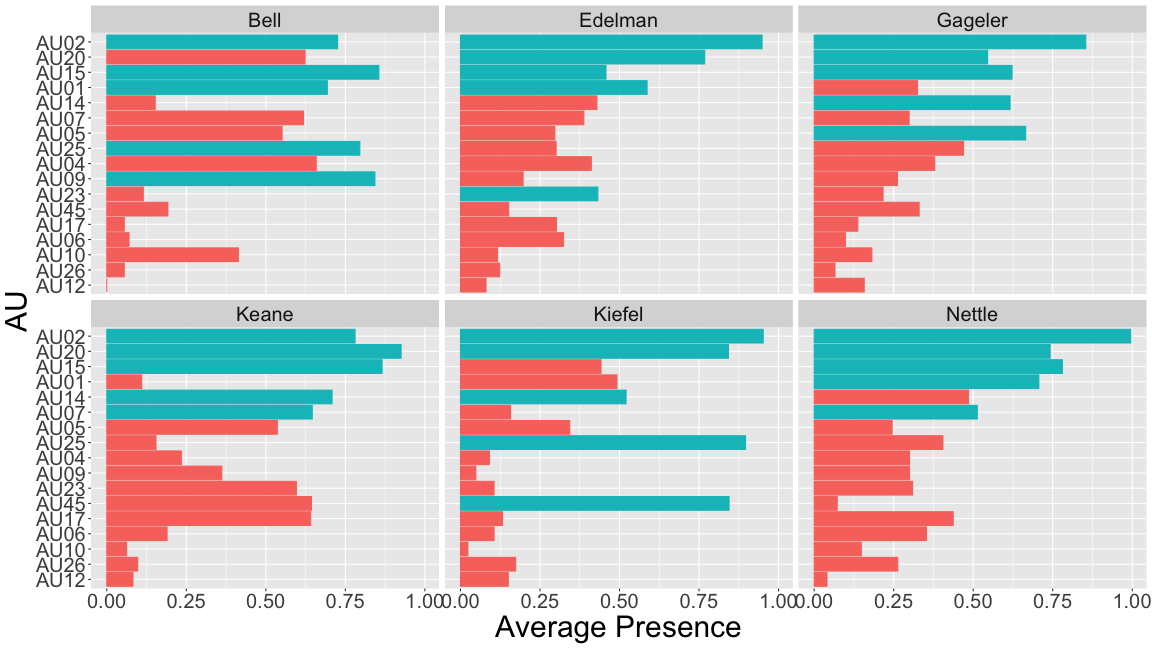
\includegraphics{Exploration_of_Judicial_Facial_Expression_in_Videos_and_Transcripts_of_Legal_Proceedings_files/figure-latex/unnamed-chunk-2-1.pdf}

The most frequent displayed action unit is highlighed in blue for each judge and summarised in the table below.

\begin{tabular}{r|l|l|l|l|l|l}
\hline
index & Bell & Edelman & Gageler & Keane & Kiefel & Nettle\\
\hline
1 & AU15 & AU02 & AU02 & AU20 & AU02 & AU02\\
\hline
2 & AU25 & AU20 & AU05 & AU15 & AU25 & AU15\\
\hline
3 & AU09 & AU01 & AU14 & AU02 & AU45 & AU20\\
\hline
4 & AU02 & AU15 & AU15 & AU14 & AU20 & AU01\\
\hline
5 & AU01 & AU23 & AU20 & AU07 & AU14 & AU07\\
\hline
\end{tabular}

It can be seen that some of the action units are common across almost all the judges, these includes

\begin{itemize}
\tightlist
\item
  AU02 (outer eyebrow raise),
\item
  AU20 (lip stretcher),
\item
  AU15 (Lip Corner Depressor) and
\item
  AU14 (Dimpler)
\end{itemize}

The table below summarises the judge specific high frequent action units.

\begin{tabular}{l|l|l|l}
\hline
judge\_id & first & second & 3\\
\hline
Bell & AU25 & AU09 & AU01\\
\hline
Edelman & AU01 & AU23 & NA\\
\hline
Gageler & AU05 & NA & NA\\
\hline
Keane & AU07 & NA & NA\\
\hline
Kiefel & AU25 & AU45 & NA\\
\hline
Nettle & AU01 & AU07 & NA\\
\hline
\end{tabular}

These are the results from inspecting the action units visually and they should also be reflected thorugh the coefficients of the relevant models {[}see stage 3 modelling{]}.

\hypertarget{presence-by-videos}{%
\subsection{Presence by videos}\label{presence-by-videos}}

Apart from visualising the general presence score for all the action unit, we are also interested in the break down statistics by video. The statistics being plotted is thus \[P_{ijk} = \frac{\sum_{t}X_{ijtk}}{T_j}\] with selected most common four action units. From this plot, it is interesting to know that almost all the judges have more frequent action units on the face for case OKS. This maybe related to the nature of the case\ldots{}

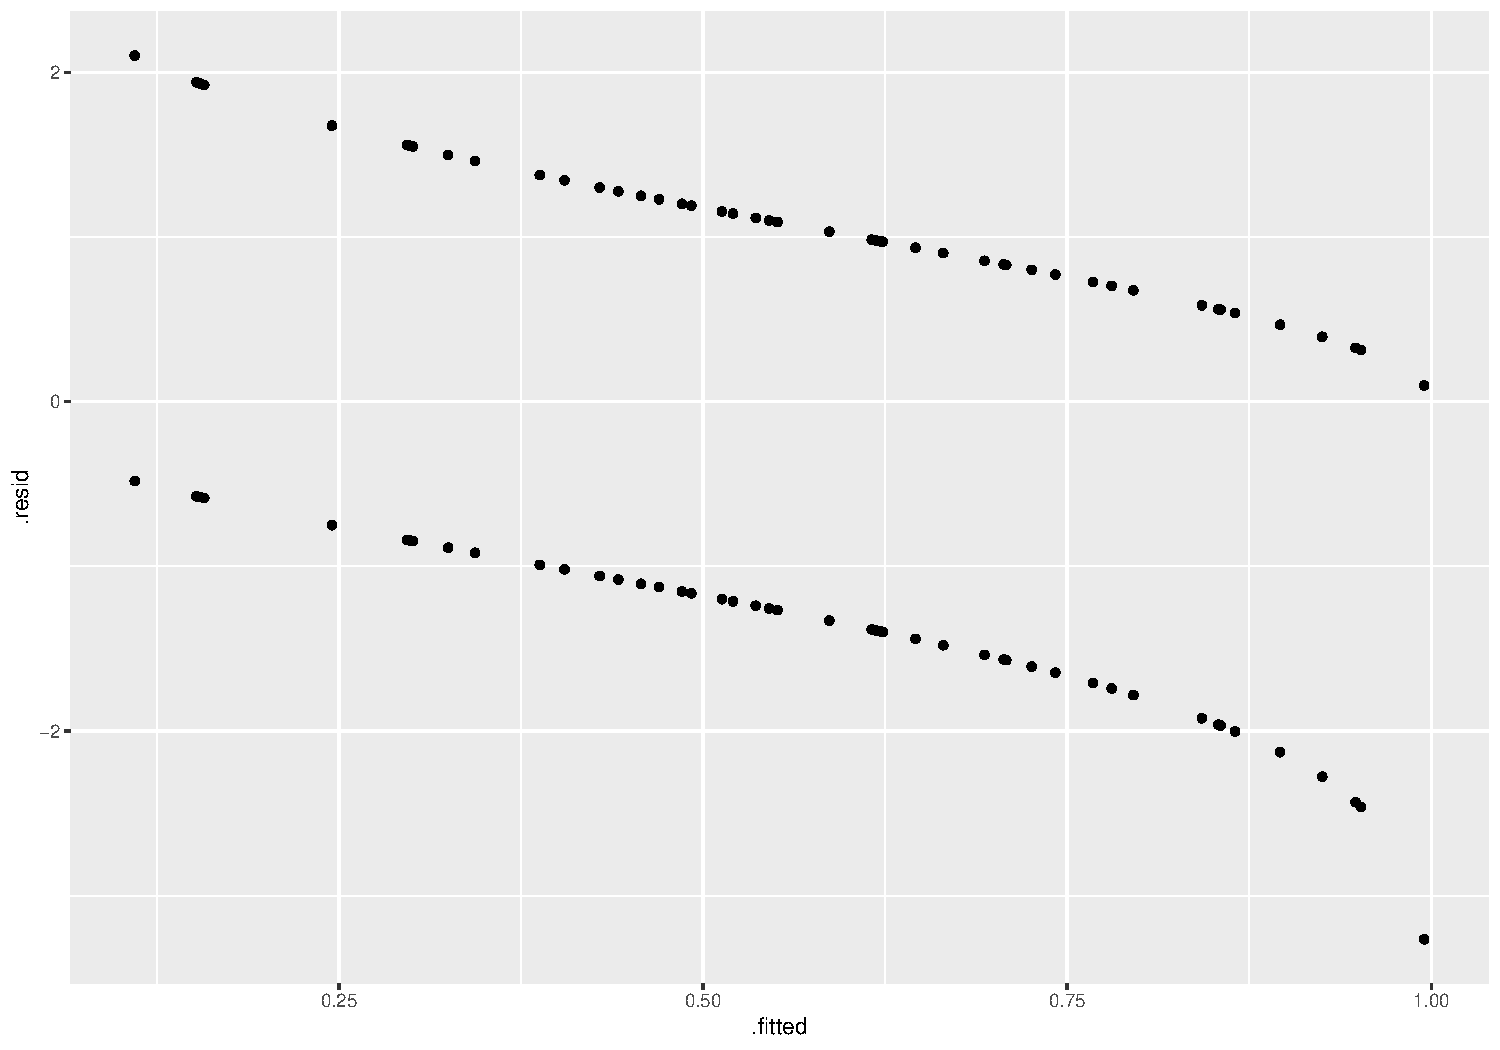
\includegraphics{Exploration_of_Judicial_Facial_Expression_in_Videos_and_Transcripts_of_Legal_Proceedings_files/figure-latex/unnamed-chunk-5-1.pdf}

\hypertarget{action-unit-intensity}{%
\section{Action unit: Intensity}\label{action-unit-intensity}}

\hypertarget{general-intensity-plot}{%
\subsection{General Intensity plot}\label{general-intensity-plot}}

The plot gives an overview of the action unit intensity of all the judges across all the trails. Each bar-and-whisker represents the intensity of all the action units aggregated on time for a particular judge in a specific case. For example, the first bar-and-whisker in case Nauru\_a is created using all the 17 action units of Edelman through out the elapsed time in Nauru\_a case. In mathematics notation, the plotted statistics is \(I_{ijtk}\) seperating by \(i \text{and} j\).

In Ekman's 20002 FACS manual, the intensity of Action unit is defined based on five classes: Trace(1), Slight(2), Marked or pronounced(3), Severe or extreme(4) and Maximum(5). From the plot, most of the action units have low intensity (almost zero average and lower than one upper bounds) and this is expected because usually in the court room, judges are expected to behave neutral. From this plot, we can see that Judge Bell doesn't seem to have many intensive expressions as we can see from the relatively small amount of dots in the whisker.

To better look at the mean of each boxplot, we take a square root transformation and hide the outliners into the upper line. We can find that Judge Nettle seems to have higher average in all the four cases he appears: Nauru\_a\&b, Rinehart\_a \&b.

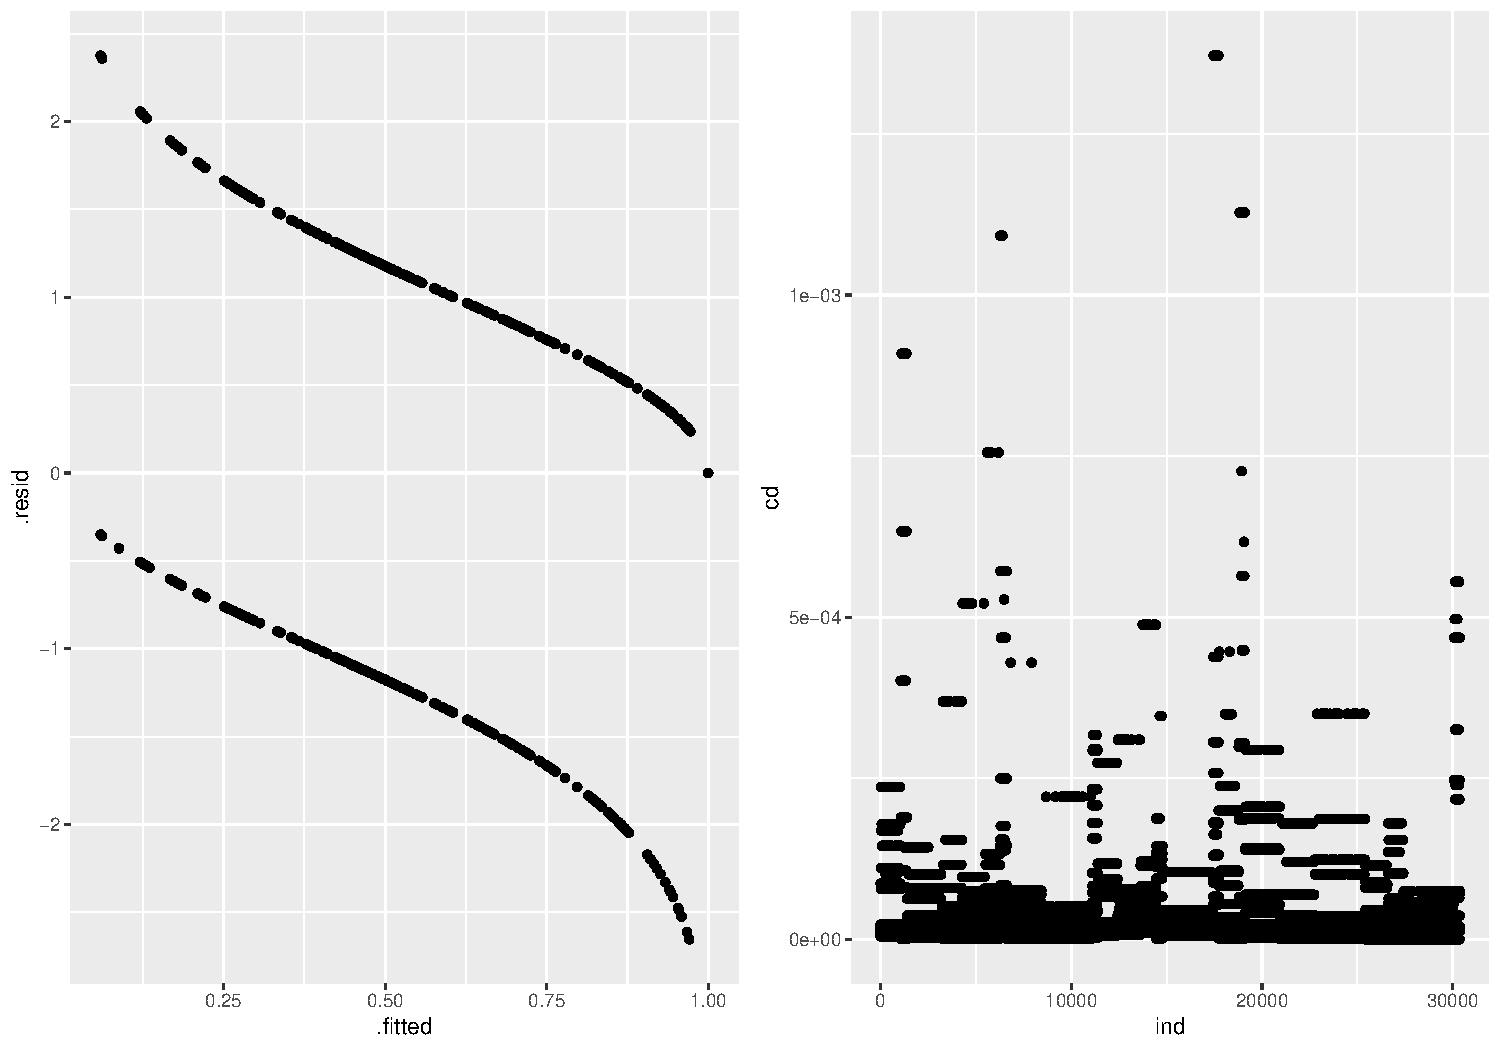
\includegraphics{Exploration_of_Judicial_Facial_Expression_in_Videos_and_Transcripts_of_Legal_Proceedings_files/figure-latex/unnamed-chunk-6-1.pdf} \includegraphics{Exploration_of_Judicial_Facial_Expression_in_Videos_and_Transcripts_of_Legal_Proceedings_files/figure-latex/unnamed-chunk-6-2.pdf}

\hypertarget{mean-intensity}{%
\subsection{Mean intensity}\label{mean-intensity}}

We compute a similar mean intensity score for each of the action unit for each of the judge, the statsitics is \[I_{ik} = \frac{\sum_{jt}X_{ijtk}}{\sum_{j = 1}^JT_j}\]. Less uniform as the mean presence plot - different judge response intense at different action units.

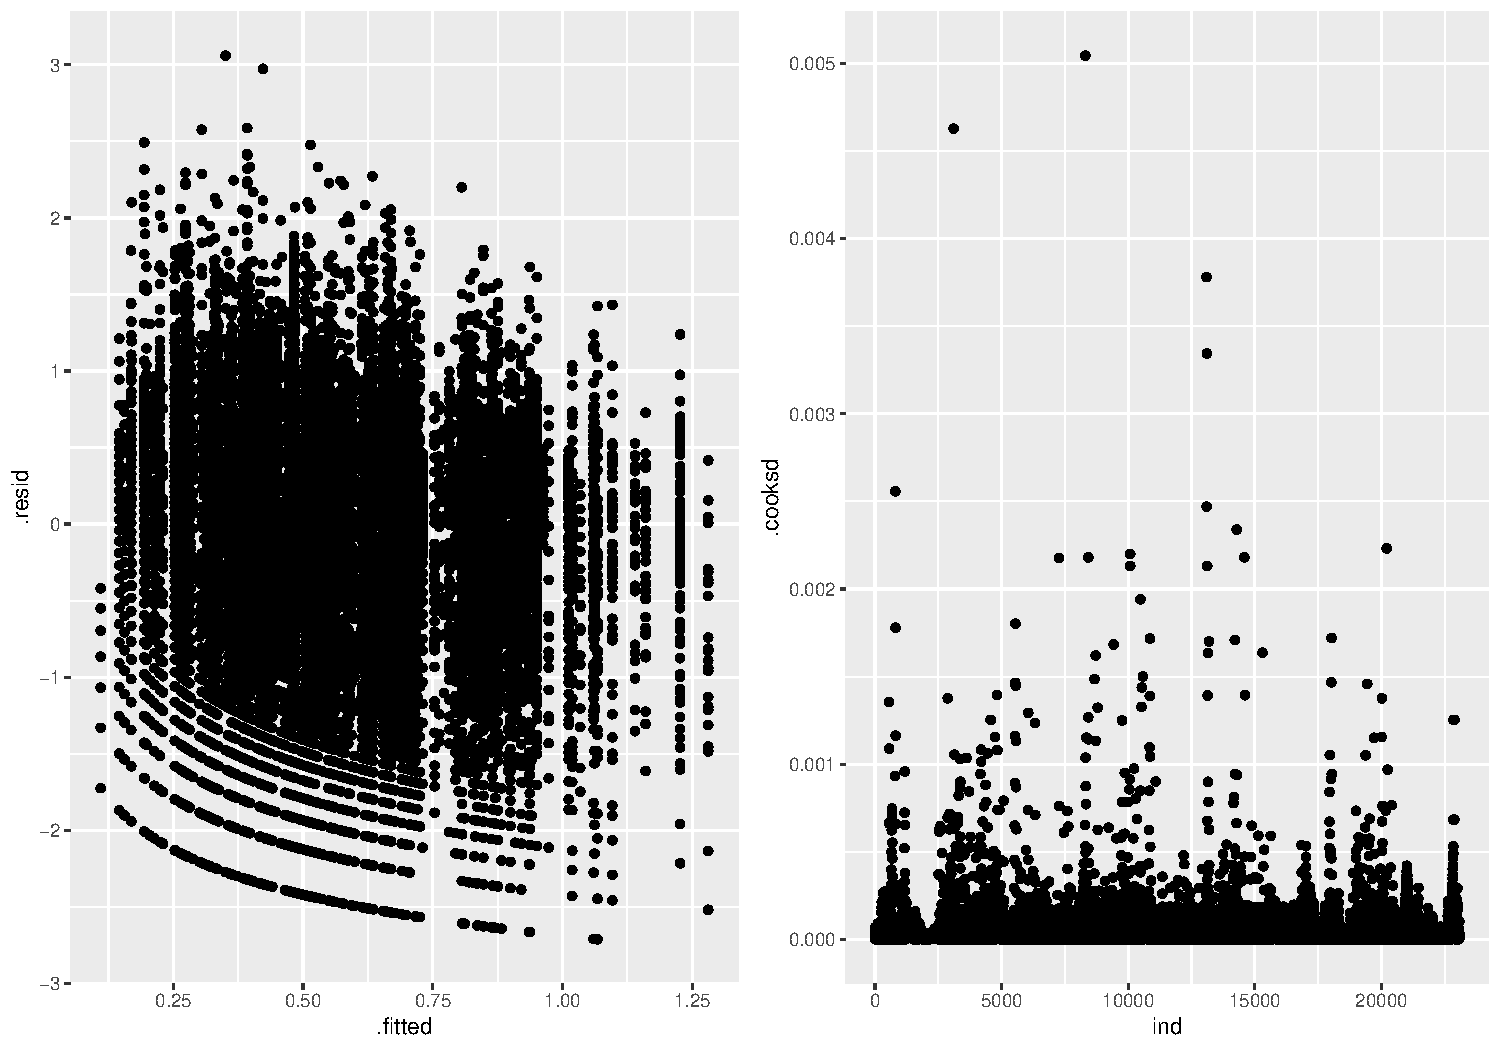
\includegraphics{Exploration_of_Judicial_Facial_Expression_in_Videos_and_Transcripts_of_Legal_Proceedings_files/figure-latex/unnamed-chunk-7-1.pdf}

\hypertarget{intensity-plot-for-the-most-frequent-action-units}{%
\subsection{Intensity plot for the most frequent action units}\label{intensity-plot-for-the-most-frequent-action-units}}

Apart from visualising the general intensity score for all the action unit, we are also interested in the intensity score of the most frequent units. The statistics being plotted is thus \(I_{ij*k}\) with selected \(i\) indicated by the \texttt{most\_common} table above. Five most frequent action units for each of the six judges give 30 subplots and I arrange them into two seperate plots: Intensity for four major high frequent action units and Intensity for other high frequent action units.

From the first plot, some panels are empty for some judges. This is because the particular action unit is not the most frequent five for that particular judge. We can learn that AU02, although being commonly detected for all the judges, the intensity is quite low.

From the second plot, most of the intensity are low as the general intensity plot, while one action unit has drawn the attention: AU45 for Kiefel. The intensity in both case parkes and case Rinehart\_a for Kiefel are relatively higher than others and this will be reflected through our model.

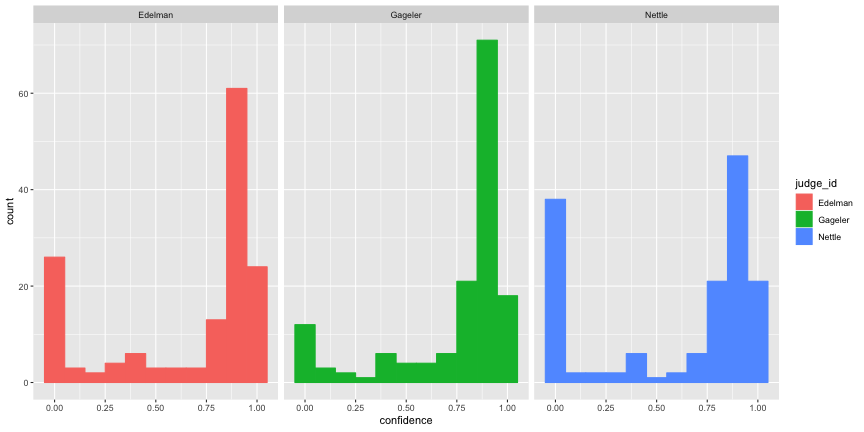
\includegraphics{Exploration_of_Judicial_Facial_Expression_in_Videos_and_Transcripts_of_Legal_Proceedings_files/figure-latex/unnamed-chunk-8-1.pdf} \includegraphics{Exploration_of_Judicial_Facial_Expression_in_Videos_and_Transcripts_of_Legal_Proceedings_files/figure-latex/unnamed-chunk-8-2.pdf}

\hypertarget{high-intensity-points}{%
\subsection{High intensity points}\label{high-intensity-points}}

We filter out the points have intensity greater than 2 (at least ``slight'' as per Ekman) in the previous plot and plot it against time and color by the speaker. It tells us that Edelman, Gageler and Nettle are the judges have stronger emotion that can be detected (since they have more points with intensity greater than 2). Different judges also have different time where they display stronger emotions. For example, Justice Nettle are more likely to have stronger emotion throughout the time when the appellant is speaking but only at the beginning and ending period when the respondent is speaking.

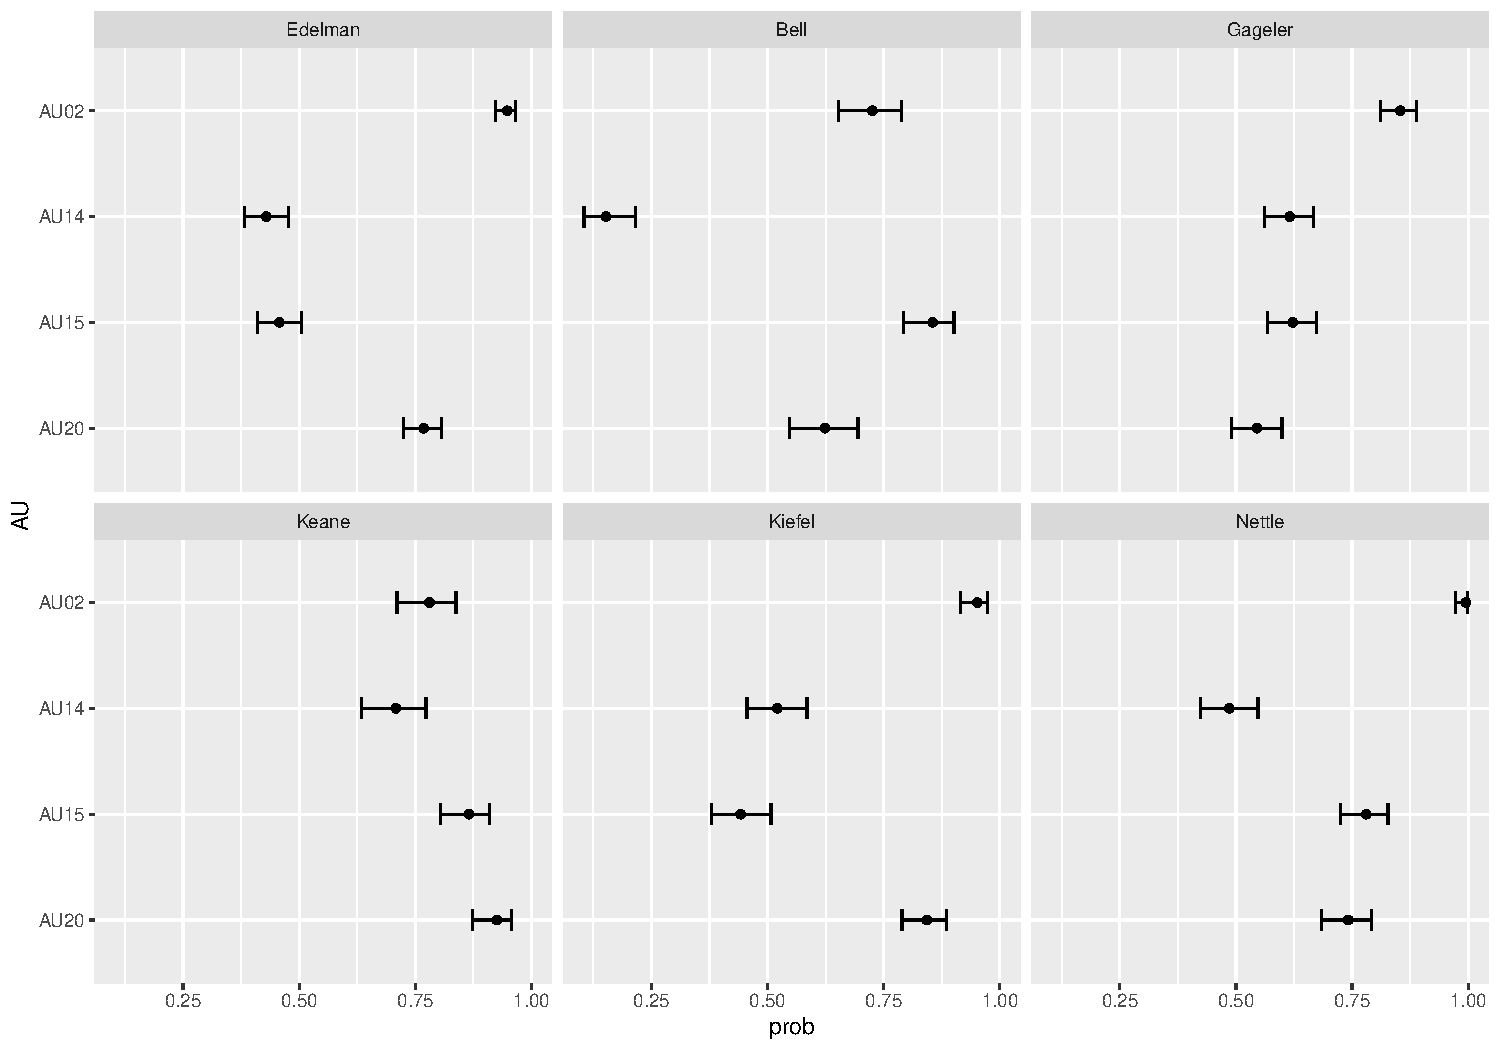
\includegraphics{Exploration_of_Judicial_Facial_Expression_in_Videos_and_Transcripts_of_Legal_Proceedings_files/figure-latex/unnamed-chunk-9-1.pdf}

\appendix

\hypertarget{additional-stuff}{%
\chapter{Additional stuff}\label{additional-stuff}}

\begin{longtable}[]{@{}lll@{}}
\caption{Details of videos processed.}\tabularnewline
\toprule
\begin{minipage}[b]{0.42\columnwidth}\raggedright
Case\strut
\end{minipage} & \begin{minipage}[b]{0.14\columnwidth}\raggedright
Name\strut
\end{minipage} & \begin{minipage}[b]{0.35\columnwidth}\raggedright
AV recording link\strut
\end{minipage}\tabularnewline
\midrule
\endfirsthead
\toprule
\begin{minipage}[b]{0.42\columnwidth}\raggedright
Case\strut
\end{minipage} & \begin{minipage}[b]{0.14\columnwidth}\raggedright
Name\strut
\end{minipage} & \begin{minipage}[b]{0.35\columnwidth}\raggedright
AV recording link\strut
\end{minipage}\tabularnewline
\midrule
\endhead
\begin{minipage}[t]{0.42\columnwidth}\raggedright
Republic of Nauru v. WET040\strut
\end{minipage} & \begin{minipage}[t]{0.14\columnwidth}\raggedright
\texttt{Nauru\_a}\strut
\end{minipage} & \begin{minipage}[t]{0.35\columnwidth}\raggedright
\url{http://www.hcourt.gov.au/cases/cases-av/av-2018-11-07a}\strut
\end{minipage}\tabularnewline
\begin{minipage}[t]{0.42\columnwidth}\raggedright
TTY167 v. Republic of Nauru\strut
\end{minipage} & \begin{minipage}[t]{0.14\columnwidth}\raggedright
\texttt{Nauru\_b}\strut
\end{minipage} & \begin{minipage}[t]{0.35\columnwidth}\raggedright
\url{http://www.hcourt.gov.au/cases/cases-av/av-2018-11-07b}\strut
\end{minipage}\tabularnewline
\begin{minipage}[t]{0.42\columnwidth}\raggedright
Rinehart \& Anor v. Hancock Prospecting Pty Ltd \& Ors on 13 Nov 18\strut
\end{minipage} & \begin{minipage}[t]{0.14\columnwidth}\raggedright
\texttt{Rinehart\_a}\strut
\end{minipage} & \begin{minipage}[t]{0.35\columnwidth}\raggedright
\url{http://www.hcourt.gov.au/cases/cases-av/av-2018-11-13}\strut
\end{minipage}\tabularnewline
\begin{minipage}[t]{0.42\columnwidth}\raggedright
Rinehart \& Anor v. Hancock Prospecting Pty Ltd \& Ors on 14 Nov 18\strut
\end{minipage} & \begin{minipage}[t]{0.14\columnwidth}\raggedright
\texttt{Rinehart\_b}\strut
\end{minipage} & \begin{minipage}[t]{0.35\columnwidth}\raggedright
\url{http://www.hcourt.gov.au/cases/cases-av/av-2018-11-14a}\strut
\end{minipage}\tabularnewline
\begin{minipage}[t]{0.42\columnwidth}\raggedright
Parkes Shire Council v. South West Helicopters Pty Limited\strut
\end{minipage} & \begin{minipage}[t]{0.14\columnwidth}\raggedright
\texttt{Parkes}\strut
\end{minipage} & \begin{minipage}[t]{0.35\columnwidth}\raggedright
\url{http://www.hcourt.gov.au/cases/cases-av/av-2018-11-14b}\strut
\end{minipage}\tabularnewline
\begin{minipage}[t]{0.42\columnwidth}\raggedright
McKell v. The Queen\strut
\end{minipage} & \begin{minipage}[t]{0.14\columnwidth}\raggedright
\texttt{McKell}\strut
\end{minipage} & \begin{minipage}[t]{0.35\columnwidth}\raggedright
\url{http://www.hcourt.gov.au/cases/cases-av/av-2018-12-07}\strut
\end{minipage}\tabularnewline
\begin{minipage}[t]{0.42\columnwidth}\raggedright
OKS v. The State of Western Australia\strut
\end{minipage} & \begin{minipage}[t]{0.14\columnwidth}\raggedright
\texttt{OKS}\strut
\end{minipage} & \begin{minipage}[t]{0.35\columnwidth}\raggedright
\url{http://www.hcourt.gov.au/cases/cases-av/av-2019-02-14}\strut
\end{minipage}\tabularnewline
\bottomrule
\end{longtable}

\begin{figure}
\hypertarget{fig:workflow}{%
\centering
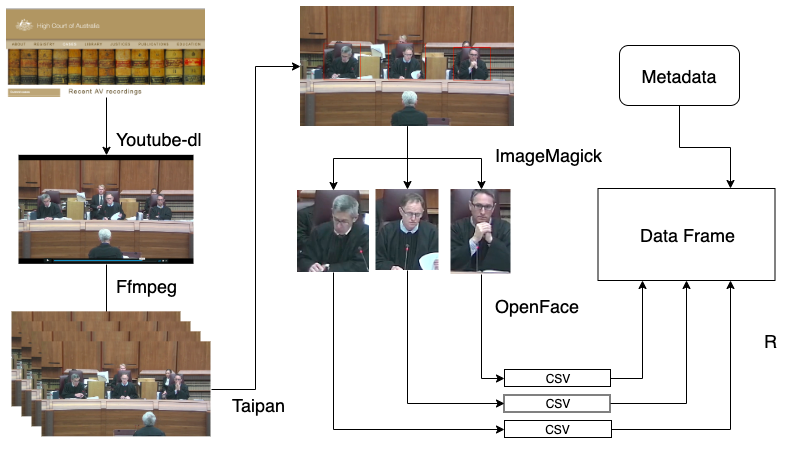
\includegraphics{figures/workflow.png}
\caption{Workflow for data extraction.}\label{fig:workflow}
}
\end{figure}

\printbibliography[heading=bibintoc]



\end{document}
